\chapter{AI: Searching Solutions}


\begin{enumerate}[itemsep=0.2cm]
    \item A solution is an action sequence, so search algorithms work by considering various possible action sequences.
    \hfill \cite{ai/book/Artificial-Intelligence-A-Modern-Approach/Russell-Norvig}

    \item The possible action sequences starting at the initial state form a \textbf{search tree} with the initial state at the root; the branches are actions and the \textbf{nodes} correspond to states in the state space of the problem. 
    \hfill \cite{ai/book/Artificial-Intelligence-A-Modern-Approach/Russell-Norvig}

    \item We consider taking various actions by \textbf{expanding} the current state; that is, applying each legal action to the current state, thereby \textbf{generating} a new set of states.
    The process of expanding nodes on the frontier continues until either a solution is found or there are no more states to expand.
    \hfill \cite{ai/book/Artificial-Intelligence-A-Modern-Approach/Russell-Norvig}

    \item \textbf{leaf node}: a node with \textbf{no} children in the tree. 
    \hfill \cite{ai/book/Artificial-Intelligence-A-Modern-Approach/Russell-Norvig}

    \item \textbf{frontier/ open list}: set of all leaf nodes available for expansion at any given point 
    \hfill \cite{ai/book/Artificial-Intelligence-A-Modern-Approach/Russell-Norvig}

    \item Search algorithms all share this basic structure; they vary primarily according to how they choose which state to expand next - the so-called \textbf{search strategy}.
    \hfill \cite{ai/book/Artificial-Intelligence-A-Modern-Approach/Russell-Norvig}

    \item Considering \textbf{loopy paths} means that the complete search tree is \textbf{infinite} because there is no limit to how often one can traverse a loop. 
    loops can cause certain algorithms to fail, making otherwise solvable problems \textbf{unsolvable}.
    \hfill \cite{ai/book/Artificial-Intelligence-A-Modern-Approach/Russell-Norvig}

    \item In some cases, \textbf{redundant paths} are \textit{unavoidable}. This includes all problems where the actions are reversible, such as route-finding problems and sliding-block puzzles.
    Following redundant paths can cause a tractable problem to become \textbf{intractable}. This is true even for algorithms that know how to avoid infinite loops.
    \hfill \cite{ai/book/Artificial-Intelligence-A-Modern-Approach/Russell-Norvig}
\end{enumerate}



\section{Designing Search Node}

\begin{figure}[H]
    \centering
    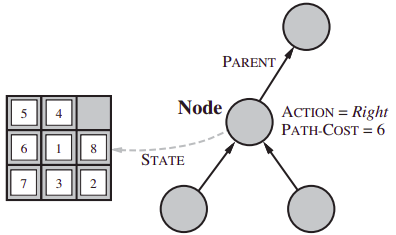
\includegraphics[
        width=0.5\linewidth,
        height=4cm,
        keepaspectratio,
    ]{images/artificial-intelligence/searching/search-node-sample.png}
    \caption*{Nodes are the data structures from which the search tree is constructed. Each has a parent, a state, and various bookkeeping fields. Arrows point from child to parent. \cite{ai/book/Artificial-Intelligence-A-Modern-Approach/Russell-Norvig}}
\end{figure}


\noindent
For each \textsc{Node} $n$ of the tree, we have a structure that contains four components:
\begin{enumerate}[itemsep=0.2cm]
    \item $n$.\textsc{State}: the state in the state space to which the node corresponds
    \hfill \cite{ai/book/Artificial-Intelligence-A-Modern-Approach/Russell-Norvig}

    \item $n$.\textsc{Parent}: the node in the search tree that generated this node
    \hfill \cite{ai/book/Artificial-Intelligence-A-Modern-Approach/Russell-Norvig}

    \item $n$.\textsc{Action}: the action that was applied to the parent to generate the node
    \hfill \cite{ai/book/Artificial-Intelligence-A-Modern-Approach/Russell-Norvig}

    \item $n$.\textsc{Path-Cost}: the cost, traditionally denoted by $g(n)$, of the path from the initial state to the node, as indicated by the parent pointers
    \hfill \cite{ai/book/Artificial-Intelligence-A-Modern-Approach/Russell-Norvig}
\end{enumerate}


\vspace{0.3cm}


\textbf{Note}:
\begin{enumerate}
    \item A node is a bookkeeping data structure used to represent the search tree. 
    A state corresponds to a configuration of the world. 
    Thus, nodes are on particular paths, as defined by \textsc{Parent} pointers, whereas states are not. 
    Furthermore, two different nodes can contain the same world state if that state is generated via two different search paths.
    \hfill \cite{ai/book/Artificial-Intelligence-A-Modern-Approach/Russell-Norvig}

    \item The \textsc{Parent} pointers string the nodes together into a tree structure. These pointers also allow the solution path to be extracted when a goal node is found.
    \hfill \cite{ai/book/Artificial-Intelligence-A-Modern-Approach/Russell-Norvig}

    \item \textsc{Solution} function is used to return the sequence of actions obtained by following parent pointers back to the root.
    \hfill \cite{ai/book/Artificial-Intelligence-A-Modern-Approach/Russell-Norvig}
\end{enumerate}










\section{General Algorithms}


\begin{algorithm}[H]
    \caption{The function \textsc{Child-Node} takes a parent node and an action and returns the resulting child node \cite{ai/book/Artificial-Intelligence-A-Modern-Approach/Russell-Norvig}}

    \SetKwFunction{FUNCTION}{\textsc{Child-Node}}
    \SetKwProg{Fn}{function}{ returns \normalfont{a \textsc{Node}}}{end}
    \Fn{\FUNCTION{problem}}{
        \Return a node with\\
            \hspace{1cm} \textsc{State} = $problem$.\textsc{Result}($parent$.\textsc{State}, $action$),\\
            \hspace{1cm} \textsc{Parent} = $parent$,\\
            \hspace{1cm} \textsc{Action} = $action$, \\
            \hspace{1cm} \textsc{Path-Cost} = $parent$.\textsc{Path-Cost} + 
                $problem$.\textsc{Step-Cost}($parent$.\textsc{State}, $action$)
    }
\end{algorithm}

\vspace{0.5cm}

\begin{algorithm}[H]
    \caption{An informal description of the general tree-search algorithm. \cite{ai/book/Artificial-Intelligence-A-Modern-Approach/Russell-Norvig}}

    \SetKwFunction{FUNCTION}{\textsc{Tree-Search}}
    \SetKwProg{Fn}{function}{ returns \normalfont{a solution, or failure}}{end}
    \Fn{\FUNCTION{problem}}{
        initialize the frontier using the initial state of problem\\
        \ \\
        \While{}{
            \If{the frontier is empty}{
                \Return failure
            }
            choose a leaf node and remove it from the frontier\\
            \If{the node contains a goal state}{
                \Return the corresponding solution
            }
            expand the chosen node, adding the resulting nodes to the frontier
        }
    }
\end{algorithm}


\vspace{0.5cm}



\begin{algorithm}[H]
    \caption{An informal description of the general graph-search algorithm. The parts of \textsc{Graph-Search} marked in bold italic are the additions needed to handle repeated states. \cite{ai/book/Artificial-Intelligence-A-Modern-Approach/Russell-Norvig}}

    \SetKwFunction{FUNCTION}{\textsc{Graph-Search}}
    \SetKwProg{Fn}{function}{ returns \normalfont{a solution, or failure}}{end}
    \Fn{\FUNCTION{problem}}{
        initialize the frontier using the initial state of problem \\
        \textbfit{initialize the explored set to be empty} \\
        \ \\
        \While{}{
            \If{the frontier is empty}{
                \Return failure
            }
            choose a leaf node and remove it from the frontier\\
            \If{the node contains a goal state}{
                \Return the corresponding solution
            }
            \textbfit{add the node to the explored set} \\
            \If{\bfseries chosen node not in the frontier or explored set}{
                expand the chosen node, adding the resulting nodes to the frontier
            }
        }
    }
\end{algorithm}


\begin{enumerate}
    \item \textbf{explored set/ closed list}: remembers every expanded node
    \hfill \cite{ai/book/Artificial-Intelligence-A-Modern-Approach/Russell-Norvig}

    \item Newly generated nodes that match previously generated nodes - ones in the explored set or the frontier - can be discarded instead of being added to the frontier. 
    \hfill \cite{ai/book/Artificial-Intelligence-A-Modern-Approach/Russell-Norvig}

    \item the search tree constructed by the \textsc{Graph-Search} algorithm contains \textbf{at most one copy} of each state, so we can think of it as growing a tree directly on the state-space graph.
    \hfill \cite{ai/book/Artificial-Intelligence-A-Modern-Approach/Russell-Norvig}

    \item The explored set can be implemented with a \textbf{hash table} to allow efficient checking for repeated states.
    \hfill \cite{ai/book/Artificial-Intelligence-A-Modern-Approach/Russell-Norvig}

    
\end{enumerate}



\section{Search Strategies/ Search Algorithms}

\subsection{Uninformed Search/ Blind Search}

\begin{enumerate}
    \item strategies have \textbf{no} additional information about states beyond that provided in the problem definition.
    \hfill \cite{ai/book/Artificial-Intelligence-A-Modern-Approach/Russell-Norvig}

    \item All they can do is generate successors and distinguish a goal state from a non-goal state. All search strategies are distinguished by the order in which nodes are expanded. 
    \hfill \cite{ai/book/Artificial-Intelligence-A-Modern-Approach/Russell-Norvig}
\end{enumerate}




\subsection{Informed Search/ Heuristic Search}

\begin{enumerate}
    \item Strategies that know whether one non-goal state is “\textit{more promising}” than another 
    \hfill \cite{ai/book/Artificial-Intelligence-A-Modern-Approach/Russell-Norvig}

    
\end{enumerate}














